%-----------------------------------------------------------------------------
%
%               Template for sigplanconf LaTeX Class
%
% Name:         sigplanconf-template.tex
%
% Purpose:      A template for sigplanconf.cls, which is a LaTeX 2e class
%               file for SIGPLAN conference proceedings.
%
% Author:       Paul C. Anagnostopoulos
%               Windfall Software
%               978 371-2316
%               paul@windfall.com
%
% Created:      15 February 2005
%
%-----------------------------------------------------------------------------


\documentclass[preprint]{sigplanconf}

% The following \documentclass options may be useful:
%
% 10pt          To set in 10-point type instead of 9-point.
% 11pt          To set in 11-point type instead of 9-point.
% authoryear    To obtain author/year citation style instead of numeric.

\usepackage{amsmath}
\usepackage[pdftex]{graphicx}
\usepackage[noend]{algorithmic}
\usepackage{algorithm,xspace,paralist}
\usepackage{wrapfig}



\newcommand{\ff}{\text{First Fit}\xspace}
\newcommand{\ffshort}{FF\xspace}
\newcommand{\ldo}{LDO\xspace}
\newcommand{\sdo}{SDO\xspace}
\newcommand{\ido}{IDO\xspace}
\newcommand{\sldo}{SDO \& LDO\xspace}
\newcommand{\gm}{G-M\xspace}
\newcommand{\etal}{\emph{et al}\xspace}
\begin{document}

\conferenceinfo{WXYZ '05}{date, City.}
\copyrightyear{2005}
\copyrightdata{[to be supplied]}

\titlebanner{banner above paper title}        % These are ignored unless
\preprintfooter{short description of paper}   % 'preprint' option specified.

\title{Evaluating Graph Coloring on GPUs}

\authorinfo{Name1\and Name2\and Name3\and Name4\and Name5}
           {Affiliation}
           {Email1/2/3/4/5}

\maketitle

\begin{abstract}
This paper evaluates features of graph coloring algorithms implemented on graphics processing units (GPUs), comparing coloring heuristics and thread decompositions.  As compared to prior work on graph coloring for other parallel architectures, we find that the large number of cores and relatively high global memory bandwidth of a GPU lead to different strategies for the parallel implementation.  Specifically, we find that a simple uniform block partitioning is very effective on GPUs and our parallel coloring heuristics lead to the same or fewer colors than prior approaches for distributed-memory cluster architecture. Our algorithm resolves many coloring conflicts across partitioned blocks on the GPU by iterating through the coloring process, before returning to the CPU to resolve remaining conflicts. With this approach we get as few color (if not fewer) than the best sequential graph coloring algorithm and we are not too far off the fastest sequential graph coloring algorithms which had poor color quality.


%Overall, parallel graph coloring speeds up well for the sparse graphs we studied, commonly yielding speedups above 1000X over a baseline CPU implementation.
\end{abstract}

%\category{CR-number}{subcategory}{third-level}

%\terms
%term1, term2, term3

\keywords
Graph coloring, Parallel algorithm, GPU, CUDA

\section{Introduction}

Graph coloring refers to the assignment of labels or colors to elements of a graph (vertices or edges) subject to certain constraints. In this paper, we consider the specific problem of assigning colors to vertices so that no two neighboring vertices (vertices connected by an edge) have the same color. There are several known applications of graph coloring like assigning frequencies to wireless access points, time-tabling and scheduling, register allocation and printed circuit testing among others.

Graph coloring is NP-hard, and even computing a $n^{1-\epsilon}$-approximation of the chromatic number of a graph is NP-hard \cite{zuckerman07}. Therefore, a number of heuristics have been developed to assign colors to vertices; some commonly used heuristics include First Fit, Largest Degree Order and Saturation Degree Order\cite{al2006new}.  These heuristics tend to trade off minimizing the number of colors and minimizing execution time but generally the faster algorithms have poor coloring quality while the slow ones tend to be better. Combinations of these algorithms have also been used to create better heuristics like the combined SDO $\&$ LDO \cite{al2006new}.

This paper examines a graphics processing unit (GPU) mapping of parallel graph coloring.  Prior parallel graph coloring algorithms have been evaluated on conventional shared-memory multiprocessors \cite{gebremedhin2000scalable} or distributed systems \cite{bozdag2008a} but to the best of our knowledge, this is the first study of how GPU architectures affect performance gains and number of assigned colors in a parallel implementation.  Our study demonstrates that features of the GPU architecture significantly impact the algorithms selected. Specifically, the support for efficient fine-grain multithreading facilitates strong performance gains over CPU implementations. Because hundreds or even thousands of threads can be applied to the parallel coloring, we can obtain as few colors as the best sequential algorithm while operating nearly as fast as the fastest sequential algorithms. 

GPUs have different architectures compared to parallel computers where most of the parallel graph-coloring algorithms are run. The main differences is that they have many processors, for example, a Tesla S1070 processor has 240 cores, but each of the cores is slower than a state-of-the-art CPU. Also, a GPU stores the data in the global memory which all the cores can readily access.




%Graph coloring refers to the assignment of labels or colors to elements of a graph (vertices or edges) subject to certain constraints. In this paper, we consider the specific problem of assigning colors to vertices so that no two neighboring vertices (vertices connected by an edge) have the same color.  There are several known applications of graph coloring like assigning frequencies to wireless access points, time-tabling and scheduling, register allocation and printed circuit testing, iterative solution of sparse linear systems [], preconditions [], sparse tiling [], and eigenvalue computation [].  

%Graph coloring is NP-hard, and even computing a $n^{1-\epsilon}$-approximation of the chromatic number of a graph is NP-hard \cite{zuckerman07}. Therefore, a number of heuristics have been developed to assign colors to vertices; some commonly used heuristics include First Fit\cite{}, Largest Degree Order\cite{} and Saturation Degree Order\cite{}.  These heuristics tend to trade off minimizing the number of colors and minimizing execution time.  Combinations of these algorithms have also been used to create better heuristics. These algorithms are generally based on the same general greedy framework: a. vertex is selected according to some predefined criteria and colored with the smallest valid color. The selection and coloring continues until all the vertices in the graph are colored.

%For coloring large graphs, a parallel implementation seems natural as we can split the graph into small subgraphs, color each of them separately in parallel, and then combine results for all of the subgraphs to derive the final coloring.   Occasionally, this combining step will encounter conflicts, where two adjacent vertices that span multiple subgraphs have been assigned the same color.  A parallel algorithm must resolve conflicts, by assigning one of the vertices involved in the conflict a different color.    Processing conflicts partially serializes the computation and may also lead to the use of a higher number of colors.

%This paper examines a graphics processing unit (GPU) mapping of parallel graph coloring.  Prior parallel graph coloring algorithms have been evaluated on conventional shared-memory multiprocessors [reference] or distributed systems [reference], but to the best of our knowledge, this is the first study of how GPU architectures affect performance gains and number of assigned colors in a parallel implementation.  Our study demonstrates that features of the GPU architecture significantly impact the algorithms selected.  Specifically, the support for efficient fine-grain multithreading facilitates strong performance gains over CPU implementations (as high as 1000X) because hundreds or even thousands of threads can be applied to the parallel coloring.  Further, multi-threading can hide the latency to memory of the irregular accesses that on a conventional CPU do not effectively utilize caches.  In addition, most parallel graph algorithms seek to partition graphs carefully to minimize the number of edges that cross processor boundaries, since cross-processor accesses typically have very high communication latencies [need a reference, possibly just a METIS reference].  On a GPU, where the entire graph is stored in a global device memory, the latency of accessing vertices inside or outside the current subgraph is no different, making the partitioning process less important. 

%Our study also identifies several features of graphs and the GPU implementation that impact both performance and number of assigned colors.  The size and sparsity of a graph affects the number of conflicts, which as suggested above, affects both performance and the quality of the coloring.  Our study evaluates parallelizing polynomial graph coloring algorithms that are known to derive fewer colors than lower complexity algorithms, but for small graphs these more efficient algorithms may also lead to the same quality solution at lower cost.  Therefore, certain graph properties determine whether using a GPU is profitable.  We will evaluate alternative coloring heuristics, partitioning strategies and granularity of the partitioning, to find the solution that leads to a high-quality coloring and a significant performance gain over a baseline CPU implementation.  We compare our coloring results to a prior parallel algorithm on the same set of graphs [from where] [reference?].

%The remainder of this paper is structured as follows: we first review previous graph coloring work will be presented.  The following section discusses the details of the parallel algorithm and the coloring heuristics we evaluated.  We present extensive experimental results followed by a conclusion.

%\section{Target platform}
%GPUs have different architectures compared to parallel computers where most of the parallel graph-coloring algorithms are run. The main differences and how they impact on algorithm are described below:
%\renewcommand{\labelenumi}{\roman{enumi}) } 
%\begin{enumerate}
% \item Number of processors: Graphics cards have many processors: an NVIDIA GTX 260 has 192 cores while a Tesla S1070 processor has 240 cores. This allows us to have much more parallelism (and having many more threads running at the same time) compared to other architectures. Moreover, as thread creation is inexpensive on a GPU, we will be running a lot to fully use the power of the GPU. Consequently our algorithm will be using many more threads than existing algorithms.
%
%\item Processor speed: While a state-of-the-art processor typically operates at around 3 GHz processor cores on GPUs are much slower: one core on a GTX 260 operates at 1242 MHz while a core on a Tesla S1070 operates between 1.296 to 1.44  GHz. Hence we need to use the many threads to match or better the speed of a standard CPU. Moreover, trying to get speedups for  O(N) algorithms are hard as the cores are individually slower and some time is wasted copying data to and from the GPU
%
%\item Memory: The memory available to parallel computers is normally bigger but it is sharing data between processors is usually much more expensive. On a GPU, all the data can be stored in the global memory and all the cores can readily access it.
%
%\end{enumerate}

%\section{ Related Work}
%In this section we give an overview of existing graph coloring algorithms, both sequential and parallel.  In this discussion, a graph $G=(V,E)$, where $V$ is a set of $n$ vertices, and $E$ is a set of $m$ edges. The degree of a vertex $v \in V$ is denoted by $d(v)$. The maximum vertex degree of a graph is denoted by $\Delta$.
%
%\subsection{Sequential greedy coloring}
%
%The problem of sequential graph coloring has been studied extensively. Among all the sequential approaches, greedy algorithms are proven to be very effective in practice, such as First Fit, Largest degree ordering, Saturation degree ordering and Incidence degree ordering[citations?]. Such greedy algorithms iterate over the vertices to be colored in a certain order, and at each step assign the current vertex the smallest permissible color. Given a graph $G$ with maximum degree $\Delta$, these procedures will use a maximum of $\Delta+1$ colors since each vertex has at most $\Delta$ neighbors. We now describe each of these greedy coloring algorithms in more detail.
%
%\begin{description}
%  \item[\ff (\ffshort):] This is the simplest algorithm of all greedy coloring heuristics\cite{klotz2002graph}. To color a vertex, a permissible color is chosen from the interval $[1,C]$, where $C$ is the largest color currently used. A new color $C+1$ is used if all  $C$ colors have been assigned to the neighbors of the vertex. \ffshort runs in time $O(m+n)$. 
%  \item[Largest degree ordering (\ldo):] \ldo first sorts vertices by degree in nonincreasing order and then runs \ff. It runs in time $O(m + n\log n)$. 
%\item[Saturation degree ordering (\sdo):] The saturation degree of a vertex is defined  as the number of different colors its neighbor vertices have been assigned. \sdo greedily picks the vertex with largest saturation degree and colors it. Since this step could change the saturation degree of other vertices, \sdo is more computationally intensive; a naive implementation takes time $O(m^2/n)$, and this can be reduced to $O(m\log n)$ using hash tables and dynamic search trees. Notice that the naive implementation runs in time $O(n^2)$ for sparse graphs.
%\item[Incidence degree ordering (\ido):] The incidence degree of a vertex is defined as the number of its adjacent colored vertices. The \ido algorithm always picks the vertex with maximum incidence degree to be colored next. It runs in time $O(m\log n)$. 
%\end{description}
%
%In general, \ff is more efficient than the other heuristics, but uses more colors. \sdo returns the fewest colors of all the heuristics\cite{gebremedhin1999parallel}, while being more expensive. Since it is often the case that many vertices have the same saturation degree, tiebreaking rules must be employed to pick the next vertex to color. A useful choice of tiebreaker is to use \ldo for tiebreaking\cite{al2006new}; Algorithm~\ref{alg:sldo} describes the resulting procedure that we term \sldo. 
%
%\renewcommand{\algorithmicrequire}{\textbf{phase}}
%\begin{algorithm}
%\caption{\sldo\label{alg:sldo}}
%\begin{algorithmic}
%\STATE {\mbox {SDO $\&$ LDO algorithm:}}
%\WHILE {$N_{colored} < n $}
%    \STATE  $ max = -1$
%    \FOR {$ i = 1\: to\: n$}
%       \IF {$!colored(v_i)$}
%           \STATE $sd = SaturatedDegree(v_i) $
%           \IF {$sd > max$}
%               \STATE $max = sd$
%               \STATE $index = i$
%           \ENDIF
%           \IF {$ sd = max$}
%             \IF {$d(v_i) > d(v_{index})$}
%                 \STATE $index = i$
%             \ENDIF
%           \ENDIF
%        \STATE $ Color \:v_{index} $
%        \STATE $N_{colored} ++$
%        \ENDIF
%    \ENDFOR
%\ENDWHILE
%\end{algorithmic}
%\end{algorithm}
%
%
%\subsection{Parallel graph coloring}
%
%A number of existing parallel algorithms are based on the concept of a maximal independent set (MIS), which is a maximal set of vertices in which no two are connected by an edge. Since all such vertices can be colored with the same color, a parallel graph coloring algorithm repeatedly finds an MIS, colors it, and then removes the vertices from the graph. Luby \cite{luby1985simple} first proposed a randomized parallel MIS algorithm that yielded an independent set in $O(\log n)$ parallel steps; this was subsequently improved by Jones  and Plassman\cite{jones1993parallel}  to $O(\log n/\log\log n)$ paralle steps for bounded-degree graphs.

% proposed by \cite{luby1985simple}. An independent set is defined as a set of vertices in which no two vertices are neighbors. For Luby’s MIS algorithm, all the vertices in an independent set are assigned to the same color, and once an independent set is found and colored, the vertices in the set and their neighbors are removed from the graph. By iterating the procedure until all the vertices in the graph are colored, the independent sets found are merged into a maximal independent set. Luby proposed a parallel algorithm of searching for an independent set based on a Monto Carlo method in \cite{luby1985simple}.

% Jones and Plassmann’s algorithm  improves the work of Luby. A single set of random weights is constructed and assigned to each vertex before coloring, and it searches for independent sets in parallel just like the MIS algorithm does, selecting the vertices with the (local) largest weights. Instead of assigning the same color to the vertices in an independent set, they are colored by the smallest color that has not been assigned to any neighbors. 

%Gjertsen\etal\cite{gjertsen1996parallel} and Allwright\etal \cite{allwright1995comparison} adapted this idea for distributed memory architectures.  Graphs are uniformly partitioned into subgraphs and each subgraph is associated with a specific processor.  To avoid color conflicts, two adjacent vertices on different processors cannot be colored in the same time step. This restriction can be overcome by Johansson’s algorithm\cite{}, where each processor is assigned a single vertex and vertices are colored randomly in the same time step. Color inconsistency may occur in this  scheme, so the coloring procedure is recursively re-run for the vertices receiving illegal colors.
%
%Gebremedhin and Manne proposed a  parallel coloring algorithm algorithm (\gm) for shared memory architectures, which achieves a linear speedup in the PRAM model \cite{gebremedhin2000scalable}. In followup work \cite{gebremedhin2006speeding} they improved the \gm algorithm by ordering the vertices to reduce cache misses and performing vertex-to-processor assignments based on graph partitioning rather than arbitrary allocation. 
%
%The \gm algorithm consists of four phases: 
%\begin{inparaenum}[(1)]
%  \item Partitioning: Assuming the number of processors is p, in this phase the graph is broken down into p independent subgraphs of almost the same size, and each subgraph is assigned to one processor. 
%  \item Pseudo-coloring: Each processor tentatively colors the vertices assigned to it in sequence. When two adjacent vertices reside on different processors are colored simultaneously, coloring inconsistency may arise.
%  \item Conflict detection:  Each processor checks the colors of  vertices assigned to it for consistency and identify a set of vertices which have color conflicts.
%  \item Conflict resolving: Re-coloring the detected vertices with conflicts.
%\end{inparaenum}

\begin{figure*}[t]
  \centering
  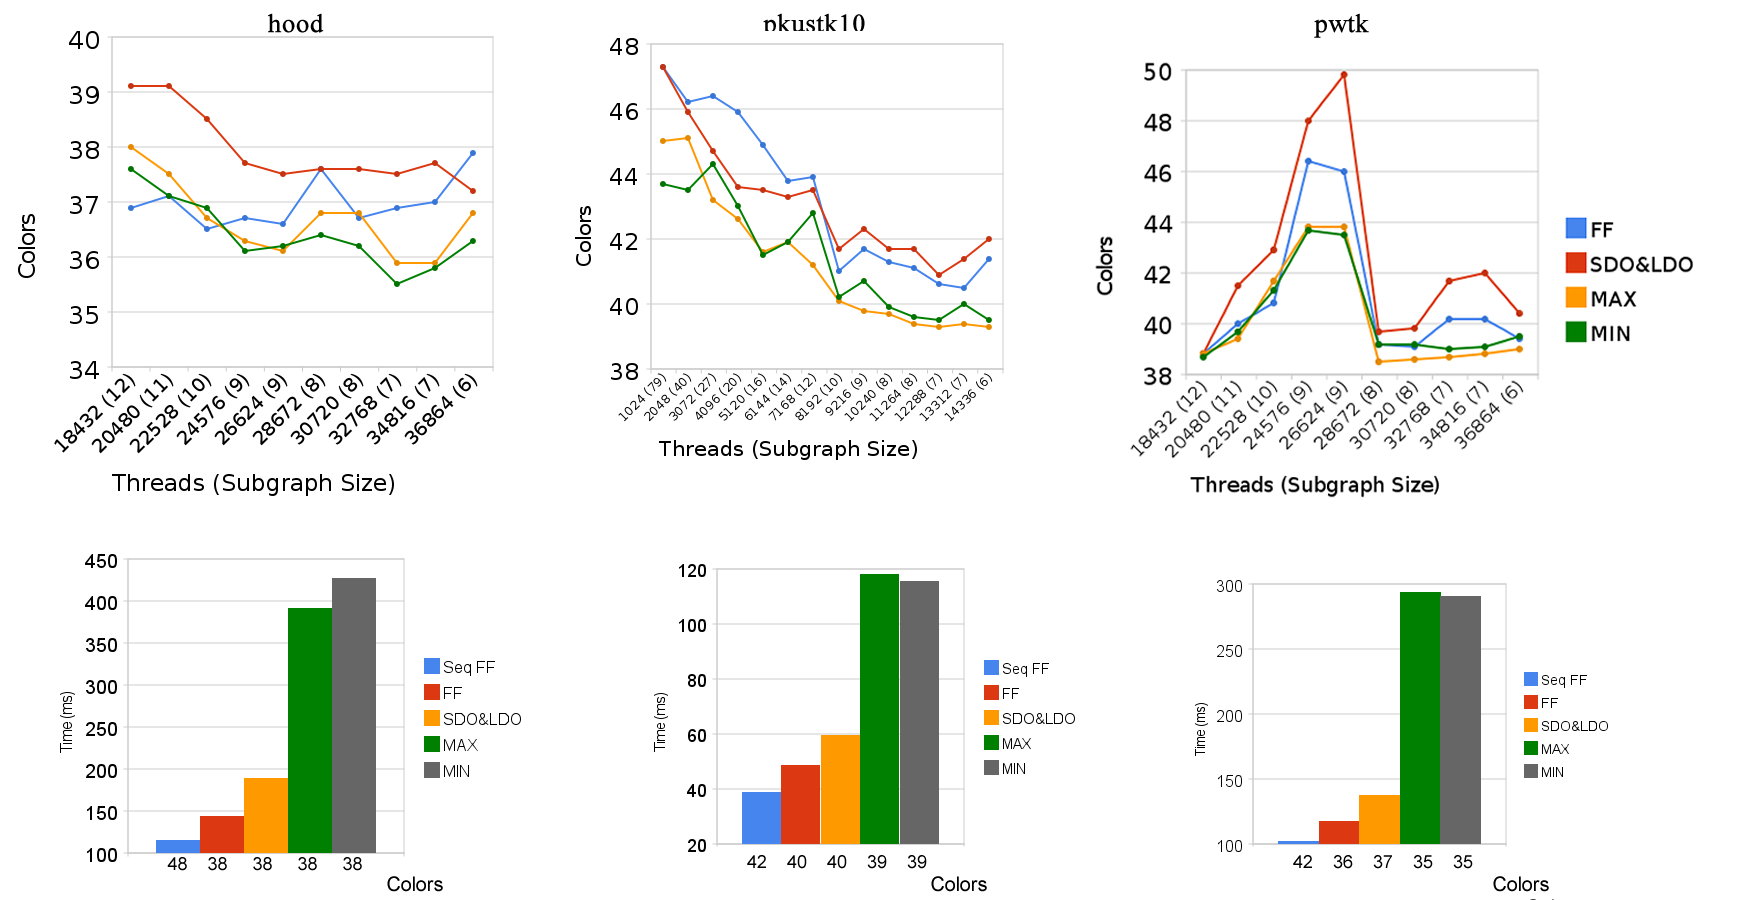
\includegraphics[scale=0.3]{figures/newPlot.png}
  \caption{ First row: Colors vs Threads (Subgraph size)  Second row: best performance for each algorithm}
  \label{fig:results}
\end{figure*}


\section{Algorithm}

In this paper, we propose a framework based on the \gm algorithm \cite{gebremedhin2000scalable}, which is adapted for an NVIDIA GPU platform.  In addition, two new heuristics are proposed to match the parallelism exploited by the GPU, which are shown to give better coloring quality than FF and  the same or better quality as SDO with the running time that is comparable to FF. 

\subsection{The Graph Coloring Framework}

\renewcommand{\algorithmicrequire}{\textbf{Phase}}
\begin{algorithm}
\caption{Graph Coloring Framework \label{alg:framework}}
\begin{algorithmic}
\REQUIRE {$1 \: : \: Graph \: Partitioning - CPU$}
    \STATE{ \mbox{Logically partition graph into subgraphs}}
	\STATE{ \mbox{Identify boundary nodes}}
	\STATE{ \mbox{Count neighbors outside the subgraph for each vertex}}
\newline
	
\REQUIRE {$2 \: : \: Graph\: Coloring $\&$ Conflict\: Solving\:- GPU$}
	\WHILE {Number of color conflicts is high}
		\STATE{ \mbox{Color graph using the specified heuristic}}
		\STATE{ \mbox{Identify color conflicts}}
		\newline
	\ENDWHILE
	

\REQUIRE {$3 \: : \: Sequential\: Conflicts\: Rsolution\: - CPU$}
	\STATE{ \mbox{Residual conflicts are eliminated}}
		
\end{algorithmic}
\end{algorithm}


\textbf{Phase 1: Graph Partitioning:}
The graph is initially padded with empty nodes so that it is exactly divisible by the total number of threads. Each thread equally takes $N/p$ vertices, which is a load-balanced approach.\\

%\textbf{Boundary Nodes:}\
%When a graph is divided into subgraphs, some of the vertices found in a subgraph have connected neighbors only in the same subgraph while others have neighbors outside.The former are referred as interior nodes and the latter are boundary nodes.Within a subgraph, the coloring procedure is conducted in sequence, so interior nodes are not likely to have color conflicts. However,since all subgraphs are colored in parallel without inter-thread communication, the boundary nodes are likely to be assigned with illegal colors conflicting with their neighbors residing in different subgraphs.  


\textbf{Phase 2: Graph Coloring $\&$ Conflicts detection:}\
Each thread assigns colors to its subgraph but checks the whole graph before allocating colors. We tried four heuristics including two proposed heuristics (MAX OUT and MIN OUT)for color allocation:
\renewcommand{\labelenumi}{\roman{enumi}) } 
\begin{enumerate}
  \item First Fit: Allocate the smallest possible color to each vertex
  \item SDO $\&$ LDO: Color is allocated to the vertex having the highest saturation and then highest degree
  \item MAX OUT: Color is allocated to the vertex having most neighbors out of the subgraph and then highest degree
  \item MIN OUT: Color is allocated to the vertex having fewest neighbors out of the subgraph and then highest degree
\end{enumerate}

Given that coloring is being performed in parallel, conflicts occur between vertices found in different subgraphs. Conflicts are identified by assigning one thread per boundary node which checks for color conflicts and reset the color of these nodes to null.\\

%For all of the 4 heuristics, when we have chosen a vertex to color, we consider all the neighbors of the latter both inside and outside the subgraph %when allocating colors.\\

%
%First Fit and SDO $\&$ LDO have already bee described in Section 3.1. We will focus on the 2 new heuristics we have devised:\\
%
%\begin{algorithm}
%\caption{Max Out Algorithm \label{alg:MAXOUT}}
%\begin{algorithmic}
%\WHILE {$N_{colored} < N $}
%    \STATE  $ max = -1$
%    \FOR {$ i = 1\: to\: N$}
%       \IF {$!colored(v_i)$}
%           \STATE $no = Number of neighbors outside partition $
%           \IF {$no > max$}
%               \STATE $max = no$
%               \STATE $index = i$
%           \ENDIF
%           \IF {$ no == max$}
%             \IF {$d(v_i) > d(v_{index})$}
%                 \STATE $index = i$
%             \ENDIF
%           \ENDIF
%        \STATE $ Color \:v_{index} $
%        \STATE $N_{colored} ++$
%        \ENDIF
%    \ENDFOR
%\ENDWHILE
%\end{algorithmic}\
%\end{algorithm}
%
%\begin{algorithm}
%\caption{Min Out Algorithm \label{alg:MINOUT}}
%\begin{algorithmic}
%\WHILE {$N_{colored} < N $}
%    \STATE  $ min = max degree$
%    \FOR {$ i = 1\: to\: N$}
%       \IF {$!colored(v_i)$}
%           \STATE $no = Number of neighbors outside partition $
%           \IF {$no < min$}
%               \STATE $min = no$
%               \STATE $index = i$
%           \ENDIF
%           \IF {$ no == min$}
%             \IF {$d(v_i) > d(v_{index})$}
%                 \STATE $index = i$
%             \ENDIF
%           \ENDIF
%        \STATE $ Color \:v_{index} $
%        \STATE $N_{colored} ++$
%        \ENDIF
%    \ENDFOR
%\ENDWHILE
%\end{algorithmic}\
%\end{algorithm}


\textbf{Phase 3: Conflicts Resolving}\
Dropping to the CPU to solve the conflicts is common in many approaches but given that we have many small partitions, we tend to have lots of conflicts and resolving that on the CPU can be quite slow. So we do multiple passes of step 2 on GPU until the number of conflicts become very small and can be quickly solved sequentially on the CPU. 


\section{Experiments and Results}
The algorithm has been implemented using the CUDA API and the tests were carried out on a Tesla S1070 with real graphs from the University of Florida Sparse Matrix Collection \cite{uofMatrix}. In this paper we will focus on 3 different graphs shown in Table~\ref{tbl:properties}



%pkustk10 & 42 & 39 & 42 & 226838 \\
%pkustk11 & 57 & 48 & 51 & 250112 \\
%pkustk13 & 57 & 66 & 51 & 612960\\


%\begin{table}
%\scriptsize
%\begin{center}
%\begin{tabular}{c c c c c}
%\hline
%Name & $n$ & $m$ & $\Delta$ & Avg Degree \
%\\
%\hline
%Structural Engineering  \\
%ct20stif & 52,329 & 1,375,396 & 206 & 50 \\
%nasasrb & 54,870 & 1,366,097 & 275 & 47 \\
%pwtk  & 217,918 & 5,926,171 & 179 & 52 \\
%\\
%Civil Engineering \\
%pkustk10 & 81,920 & 2,114,154 & 89 & 52 \\
%pkustk11 & 87,804 & 2,565,054 & 131 & 55 \\
%pkustk13 & 94,893 & 3,260,967 & 299 & 68\\
%\\
%Automotive \\
%hood & 220,542 & 5,273,947 & 76  & 47 \\
%msdoor & 417,792 & 9,912,536 & 76 & 46 \\
%ldoor & 958,464 & 22,785,136 & 76 & 46 \\
%
%\end{tabular}
%\caption{Graph properties and source}
%\label{amean_time}
%\end{center}
%\end{table}
%
%
%
%Say more about the graphs.  Range of similar average degree.  Variation in max-degree and size.  Similar number of colors, but size impacts execution time significantly due to polynomial algorithm.  etc. etc.
%  
%
%Sequential First Fit and SDO $\&$ LDO were run on each of the above graphs to get a color and timing baseline.  
%    
%\begin{table}
%\scriptsize
%\begin{center}
%\begin{tabular}{l c c c c}
%\hline
%Name & Colors  & Time  & Colors & Time \\
% & FF & FF &   SDO$\&$LDO &  SDO$\&$LDO\
%\\
%\hline
%ct20stif & 49 & 29 & 48 & 203387 \\
%nasasrb & 41 & 29 & 36 & 646113 \\
%pwtk  & 48 & 116 & 48 & 5000000 \\
%\\
%pkustk10 & 42 & 39 & 42 & 226838 \\
%pkustk11 & 57 & 48 & 51 & 250112 \\
%pkustk13 & 57 & 66 & 51 & 612960\\
%\\
%hood & 42 & 105 & 36  & 1709180 \\
%msdoor & 42 & 197 & 35 & 7281740 \\
%ldoor & 42 & 450 & 35 & 34584800 \\
%
%\end{tabular}
%\caption{Sequential coloring results for FF and SDO$\&$LDO}
%\label{amean_time}
%\end{center}
%\end{table}


%While the colors are accurate, the timing information for the sequential SDO $\&$ LDO could have been improved. The latter has is from a naive implementation which is quite inefficient. Nevertheless, the sequential SDO $\&$ LDO has been reported by its authors [...] to be O (N$^2$) and despite yielding a good coloring is quite slow. On the other hand, First Fit which is fast yields a poor coloration!\
%Ideally what we would really want is a fast algorithm that generates as few colors as possible.

\begin{table}[!ht]
\scriptsize
\begin{tabular}{c c c c c c c c }
\hline
  &   &  &  \multicolumn{3}{c}{Colors} &  \\
Name & $n$ & $m$ & $\Delta$ & FF & SDO $\&$ LDO & FF Time \
\\
\hline
hood & 220,542 & 5,273,947 & 76 & 42 & 36 & 104.7\\
pkustk10 & 81,920 & 2,114,154 & 89 & 42 & 42 & 39\\
pwtk & 217,918 & 5,926,171 & 179 & 57 & 48 & 48\\
\end{tabular}
\caption{Graph properties - $n$: number of vertices, $m$ the number of edges $\&$ $\Delta$: maximum vertex degree}
\label{tbl:properties}
\end{table}



To investigate the impact of parallel graph coloring algorithms on  both performance and number of colors obtained, the number of threads is linearly incremented and the timing and color obtained is compared and the results are shown in Figure ~\ref{fig:results}\\

The results show how different algorithms affect the number of colors and performance as a function of the number of threads. MAX and MIN generally yield fewer colors than any other algorithm and we also notice that good coloration is obtained at relatively small graph sizes.
In terms of speed among the parallel graph coloring algorithms, First Fit is the fastest followed by SDO $\&$ LDO and MIN and MAX which take the same amount of time.

%\textbf{Number of threads}\
%Given that the graphs have very different sizes, it does not make sense to use the same number of threads for each. For example, for a graph of 50 000 nodes, if 1024 threads are used, each thread handles about 48 vertices while for a graph of 500 000 nodes, each thread will operate on around 480 vertices. Since GPU cores are much slower than state-of-the-art processors speedup gains are the result of using as many cores as possible where each is operating on just a few vertices.
%
%To determine subgraph sizes that tend to give fewer colors, we linearly decreased the size of the subgraph by varying the number of threads for each of the 9 real graphs that we have. The results is shown in Figure~\ref{figureSubGraph} and Table~\ref{optimalColoringTable}.\\
%
%\begin{figure}
%  \centering
%  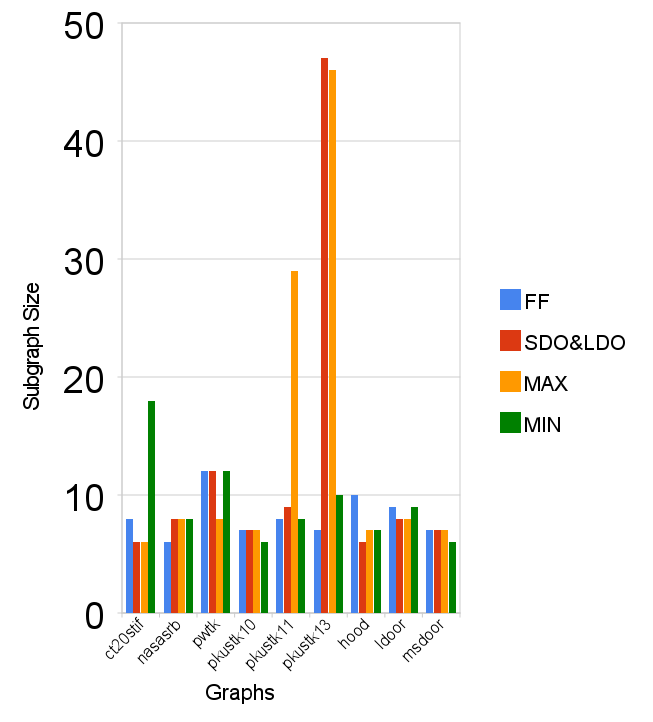
\includegraphics[scale=0.5]{figures/subgraphSize.png}
%  \caption{Subgraph size for Optimal color per algorithm and graph}
%  \label{figureSubGraph}
%\end{figure}
%
%
%
%\begin{table}
%\scriptsize
%\begin{center}
%\begin{tabular}{c c c}
%\hline
%Parallel Algorithm  & Average  & Standard Deviation \\
%\hline
%FF & 8.2 & 1.9 \\
%SDO$\&$LDO & 12.2 & 13.2 \\
%MAX OUT & 14.0 & 14.0 \\
%MIN OUT & 9.3 & 3.8 \\
%\end{tabular}
%\caption{Subgraph size for optimal coloring}
%\label{optimalColoringTable}
%\end{center}
%\end{table}


%
%\subsection{Multi Passes}\
%In the second set of experiments, we allow the program to determine the number of GPU passes it requires. We have seen that if the CPU has fewer than 200 conflicts to solve it is very fast(It is better to use a percentage, like percentage of the total number of vertices, but the stop criterion dose not have math ). (How did you arrive at this number of 200?)  - can we instead say that we move over to CPU when the number of remaining conflicts is negligible So after each pass we check to see the number of conflicts and if it is approximately less than 200, we terminate the GPU Passes and send the remaining conflicts to the CPU for solving.\

%\begin{figure*}[h]
%  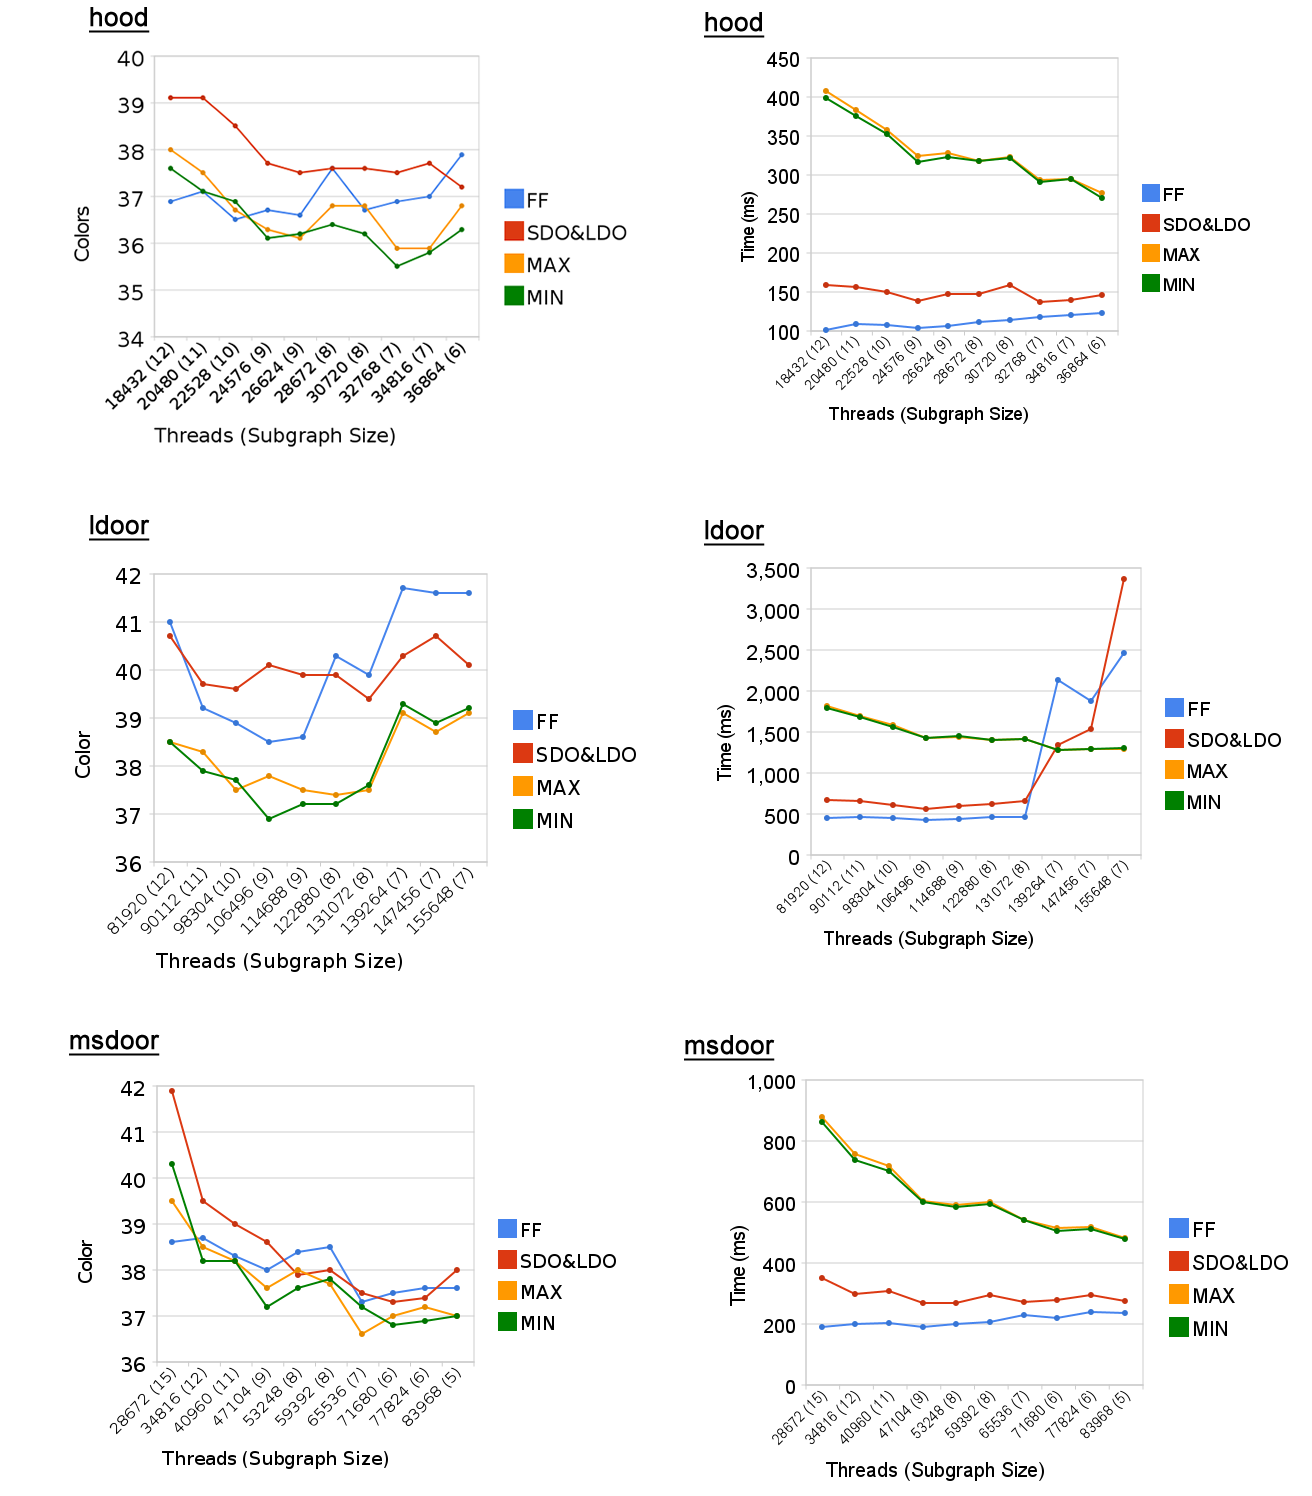
\includegraphics[scale=0.4]{figures/automotive.png}
%  \caption{ Automotive }
%\end{figure*}
%
%\begin{figure*}[h]
%  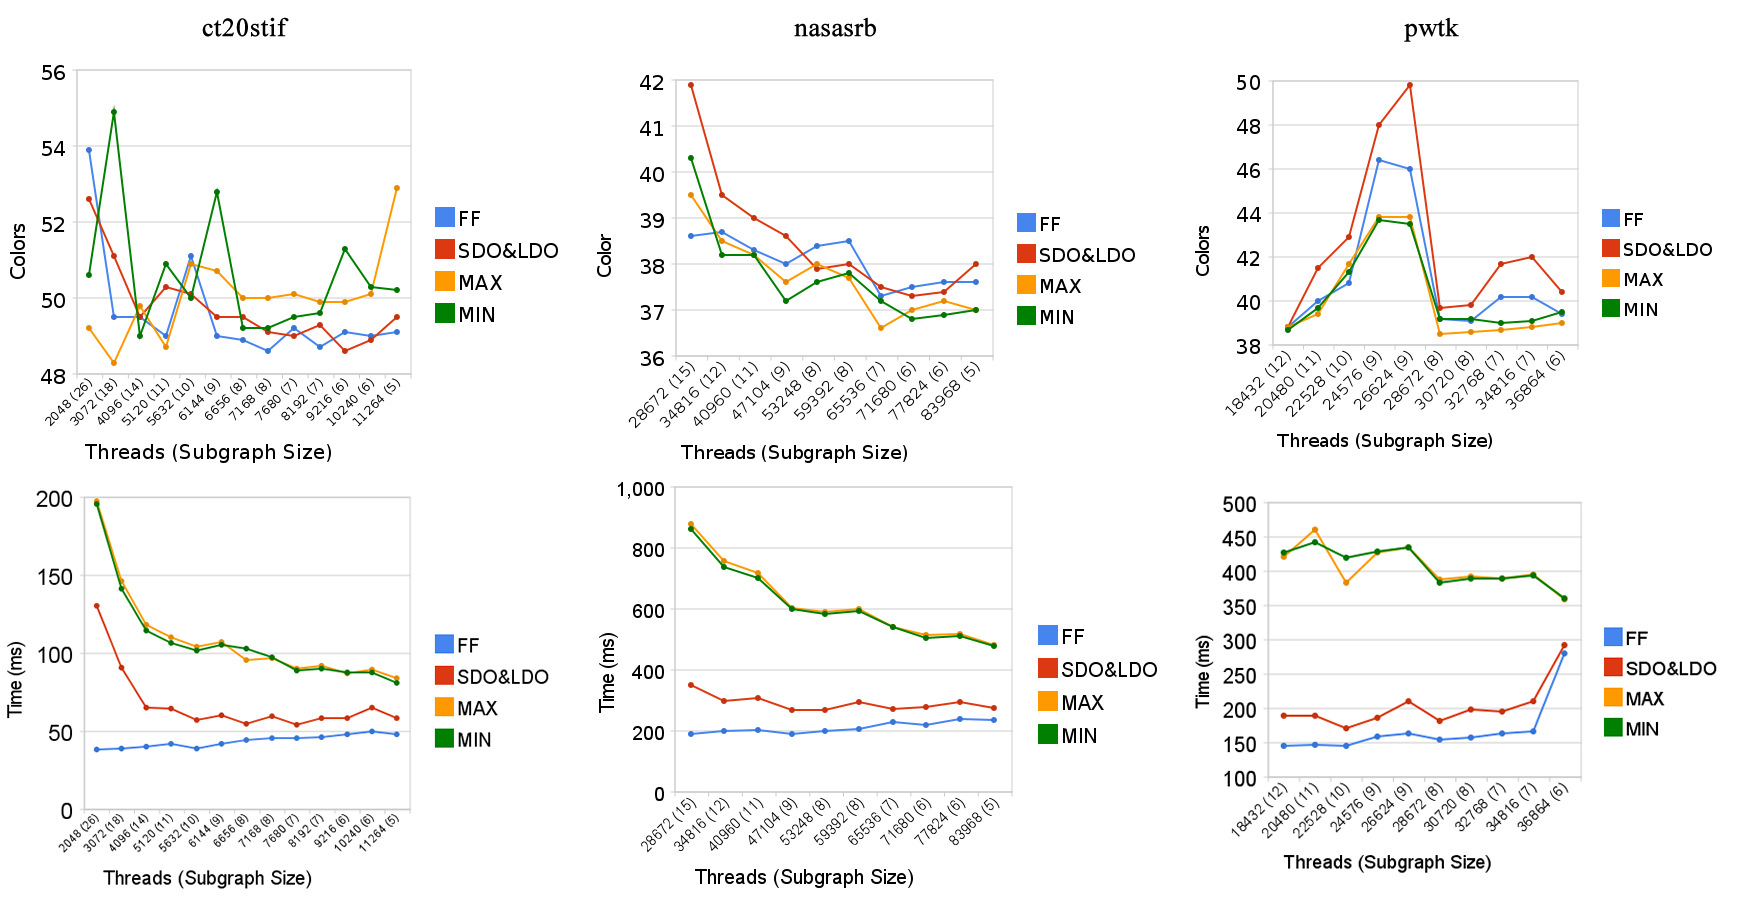
\includegraphics[scale=0.3]{figures/structuralLand.png}
%  \caption{ Structural }
%\end{figure*}


%
%\begin{figure*}[h]
%  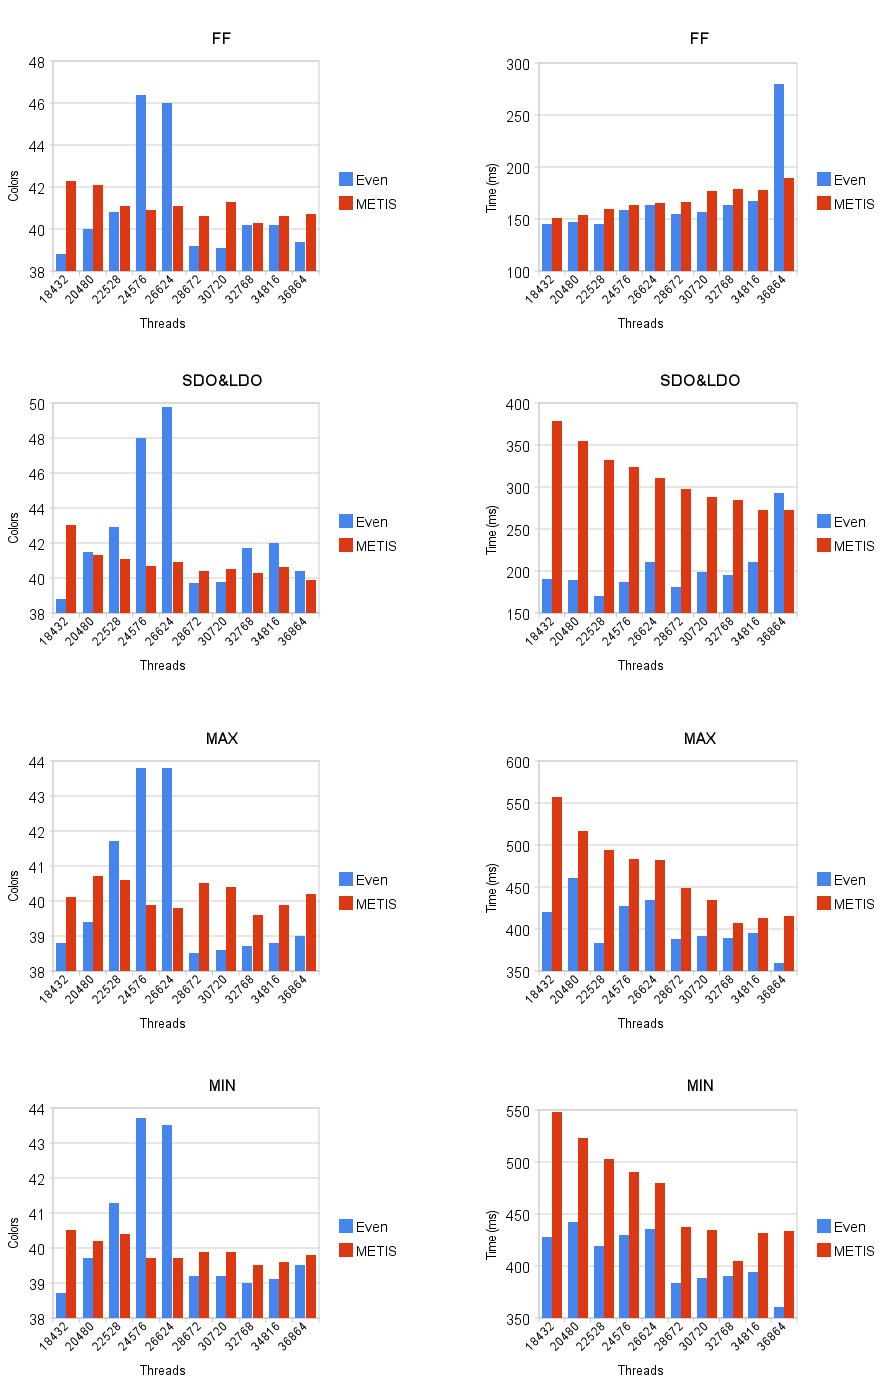
\includegraphics[scale=0.45]{figures/pwtkMetis.png}
%  \caption{ Pwtk Metis }
%\end{figure*}
%
%\begin{figure*}[h]
%  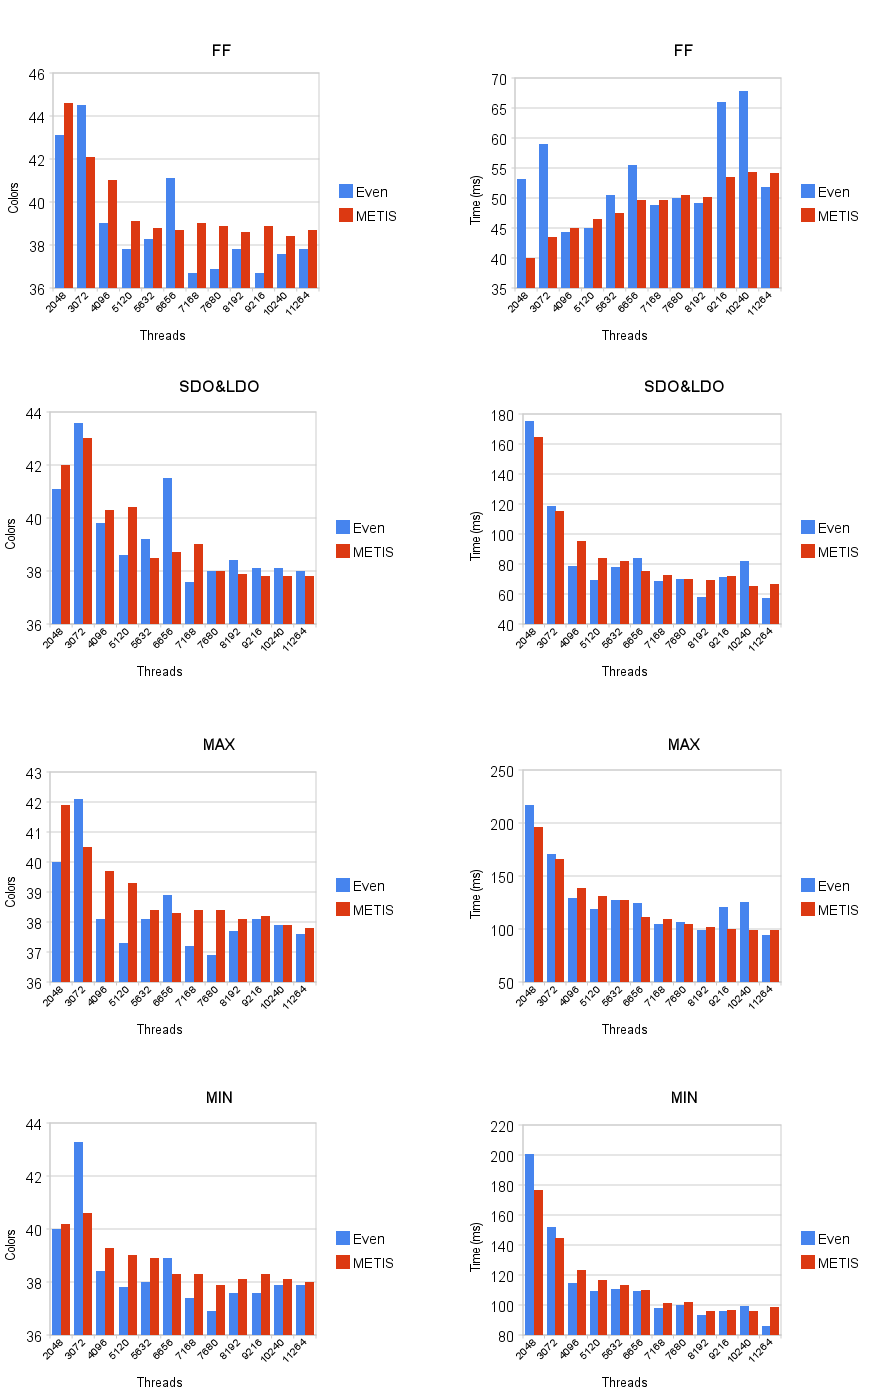
\includegraphics[scale=0.45]{figures/nasasrbMetis.png}
%  \caption{ Nasasrb Metis }
%\end{figure*}
%
%Refer to the figures.  Need better labels (graph names rather than a,b,c).  SDO$\&$LDO is approximately twice as fast as compared to MAX or MIN. However, the number of colors for MAX and MIN is usually better than SDO$\&$LDO, with MAX nearly consistently yielding  fewer colors. For this set of graphs, the MAX heuristic also yields fewer colors that the sequential SDO$\&$LDO algorithm and the sequential First Fit   (FF: 42, 57, 57 - SDO: 42, 51, 51 - Best form other Paper: 44, 57,57 removed)  Also should talk about relationship between number of threads and colors, and number of threads and performance.  Where in these graphs does the performance associated with 8 vertices per subgraph fall?  Need to make a connection back to that.\
%
%For this second set of tests, we see that though we easily beat the sequential First Fit in terms of color allocated, for ct20stif and nasasrb, we do not get consistently get fewer or match the colors of sequential SDO$\&$LDO while for the pwtk graph, we are well below the 48 colors obtained from running sequential SDO.  Do you have a sense why you are using fewer colors?
%
%For ct20stif, in our 10 test runs we sometimes get 47 colors which beat the sequential SDO implementation but on average we get more colors and the best performances are obtained with parallel First Fit. Where is non-determinism coming from?  The conflict resolution?  You should probably elaborate on that.
%(FF: 50, 47, 52 - SDO: 48, 36, 48 - Best from other Paper: 47,38,41)\
%
%\subsection{Using METIS}
%METIS is a set of algorithms that can be used to partition a graph into subgraphs. Many parallel graph algorithms advise the use of METIS to have better partitioning. However these algorithms run on parallel machines and they do not divide graphs in as many partitions as we do. Consequently when we tried to run METIS to partition the graph as we need, the resulting partitions were very unbalanced. The figure below shows the subgraph sizes from metis.


\section{Conclusion}
Though our GPU implementation is slower than the reported fastest Sequential Graph Coloring algorithm, in terms of color quality, we are much better; we sometimes even beat the sequential SDO $\&$ LDO as well as colors reported in \cite{bozdag2008a}.


%\appendix
%\section{Appendix Title}
%
%This is the text of the appendix, if you need one.
%
%\acks
%
%Acknowledgments, if needed.

% We recommend abbrvnat bibliography style.

\bibliographystyle{abbrvnat}
\bibliography{reference}

% The bibliography should be embedded for final submission.

%\begin{thebibliography}{}
%\softraggedright

%\bibitem[Smith et~al.(2009)Smith, Jones]{smith02}
%P. Q. Smith, and X. Y. Jones. ...reference text...




%\end{thebibliography}

\end{document}

